% !TEX program = xelatex

\documentclass{beamer}
\usepackage{graphicx}
\usepackage{caption}
\usetheme{metropolis} % Use trigon theme
% \trigonset{titlestyle=style2} % Use style
\captionsetup[figure]{font=tiny,labelfont=tiny} % Set caption font size

% Set title page info
\title{Participez à un concour sur la smartcity}
\subtitle{AI Engineer - Projet 2}
\date{\today}
\author{Ludovic Lafon}
\institute{OpenClassrooms}

% Begin document
\begin{document}
\maketitle
\tableofcontents
% Exploration des données
\section{Exploration des données}
% Nombre de données par colonnes
\begin{frame}{Nombre de données par colonnes}
	\begin{figure}
		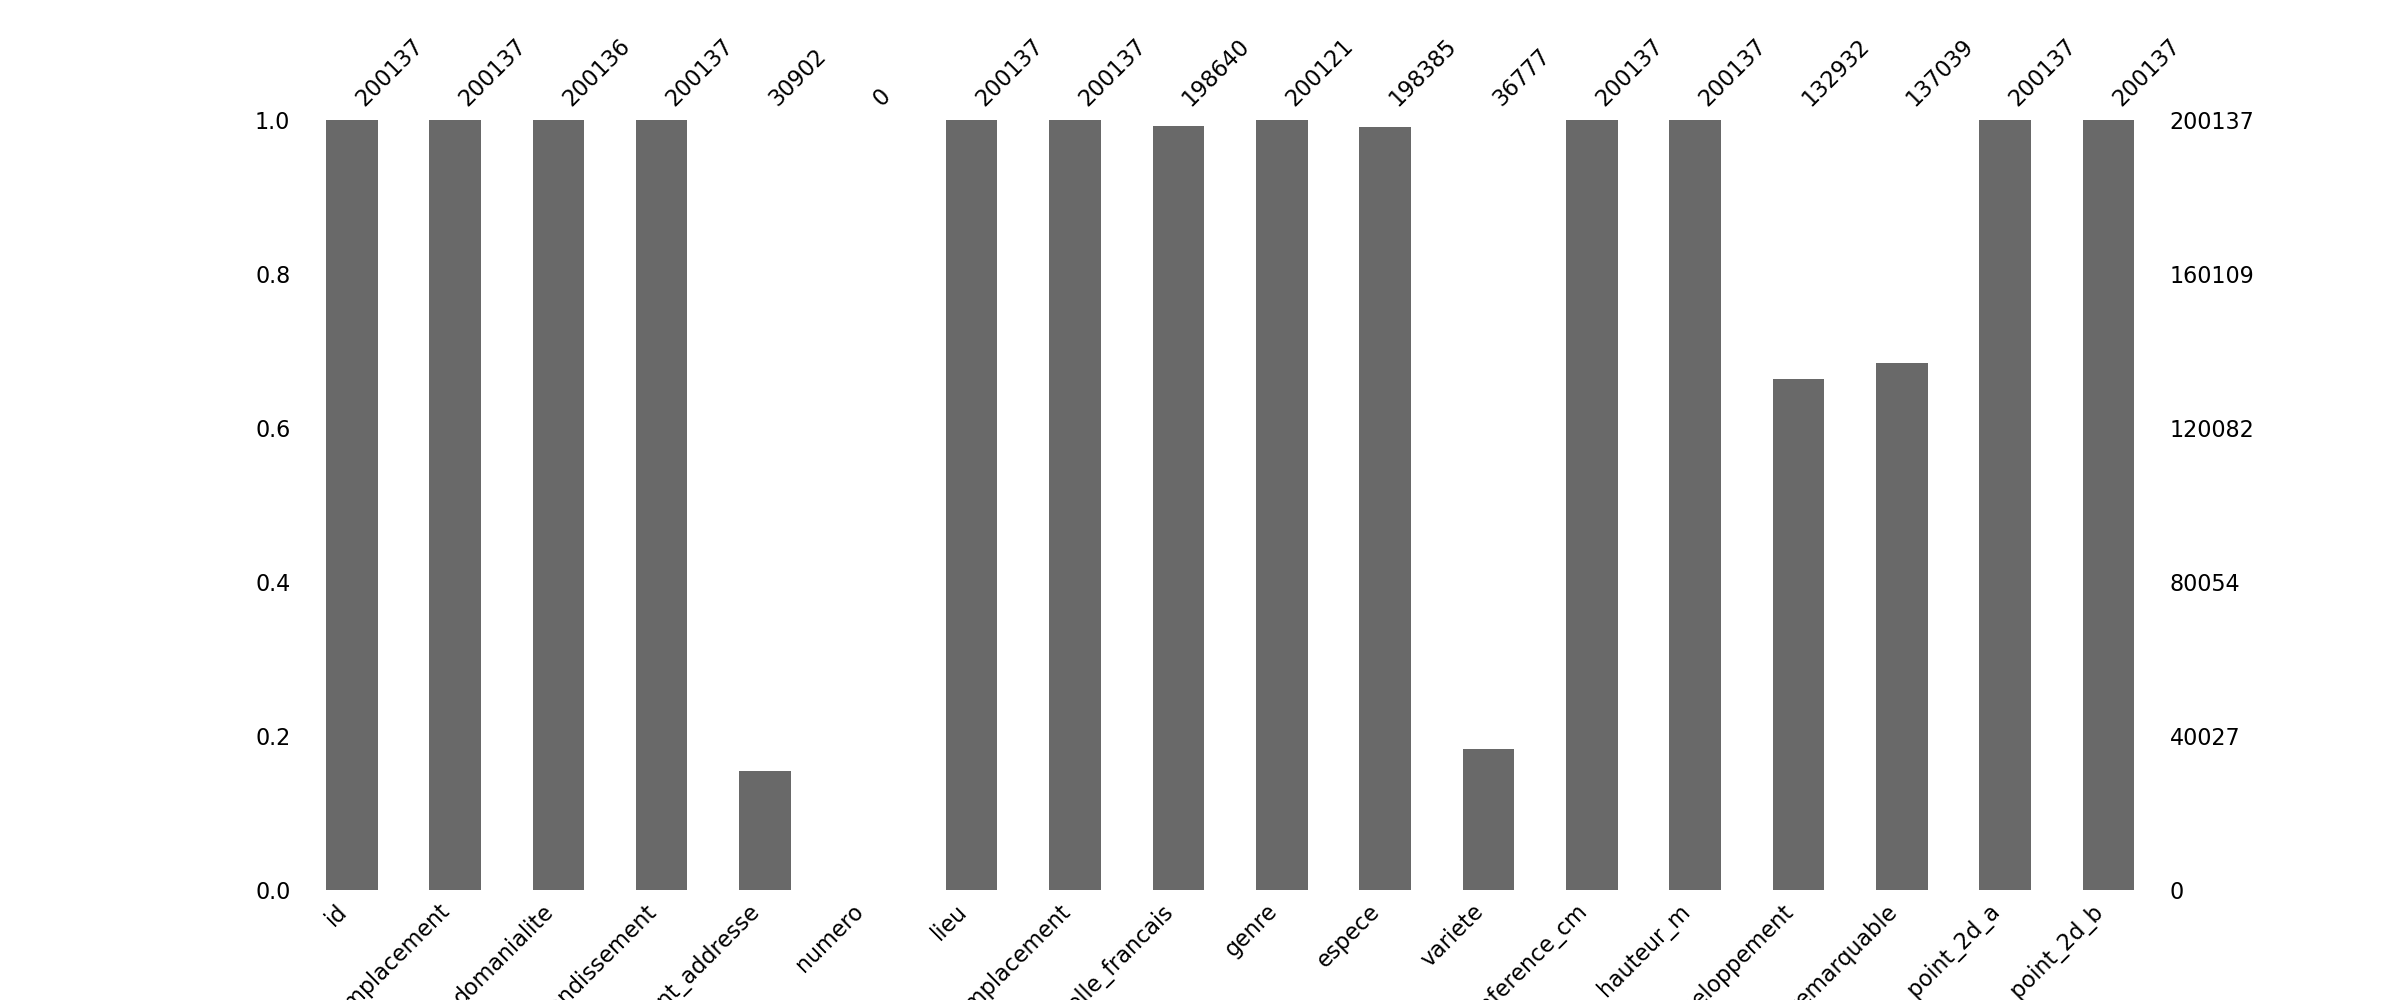
\includegraphics[width=\textwidth,height=0.6\textheight,keepaspectratio]{ressources/missingno1.png}
			\caption{Nombre de données par colonnes}
	\end{figure}
	\begin{figure}
		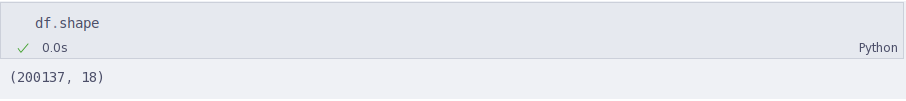
\includegraphics[width=0.80\textwidth,keepaspectratio]{ressources/dfinfo1.png}
			\caption{pandas.DataFrame.shape() - 200137 lignes, 18 colonnes}
	\end{figure}
\end{frame}
% Données manquantes
\begin{frame}{Données Manquantes}
	\begin{columns}
	\begin{column}{0.2\textwidth}
		\tiny
		Données manquantes :
		\begin{itemize}
			\item domanialite
			\item complement addresse
			\item numero
			\item libelle francais
			\item genre
			\item espece
			\item variete
			\item stade developpement
			\item remarquable
		\end{itemize}
	\end{column}
	\begin{column}{0.9\textwidth}
		\begin{figure}
		\centering
		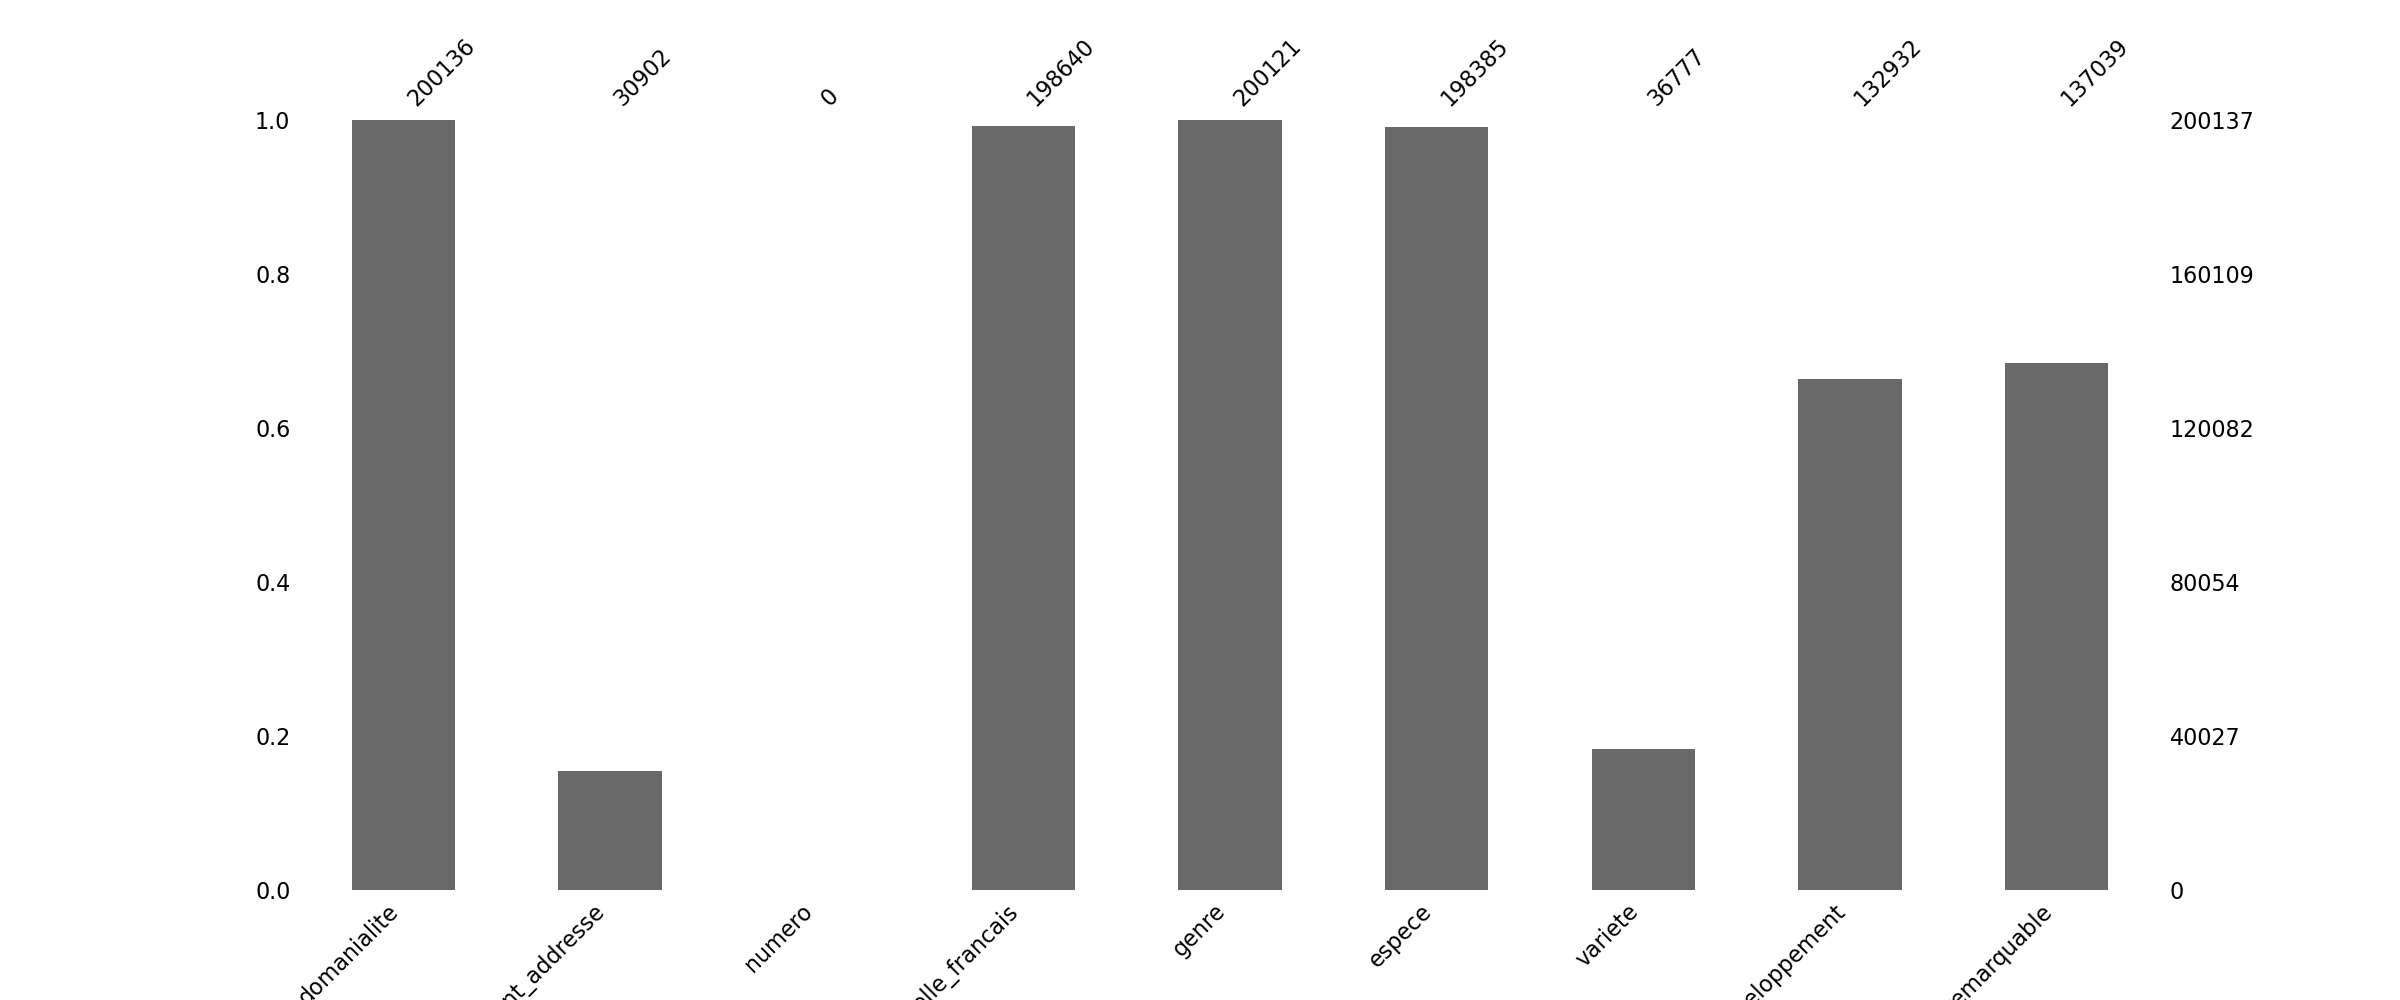
\includegraphics[width=\textwidth,keepaspectratio]{ressources/missingno2.png}
			\caption{Nombre de données par colonnes pour les colonnes non intégralement remplies}
		\end{figure}
	\end{column}
	\end{columns}
	\begin{columns}
	\begin{column}{0.4\textwidth}
		\begin{alertblock}{Une colonne est vide !}
			\begin{itemize}
				\item numero
			\end{itemize}
		\end{alertblock}
	\end{column}
	\begin{column}{0.6\textwidth}
		\begin{alertblock}{Deux colonnes sont presque vide !}
			\begin{itemize}
				\item complement addresse
				\item variete
			\end{itemize}
		\end{alertblock}
	\end{column}
	\end{columns}
\end{frame}

% Données Géographiques
\begin{frame}{Données Géographiques}
	\begin{itemize}
		\item domanialite
		\item arrondissement
		\item complement addresse
		\item lieu
		\item geo point 2d a
		\item geo point 2d b
	\end{itemize}
\end{frame}
\begin{frame}{Données Géographiques}
	\begin{columns}
	\begin{column}{0.5\textwidth}
		Colonnes gardée :\\
		\begin{itemize}
			\item domanialite
			\item arrondissement
			\item geo point 2d a
			\item geo point 2d b
		\end{itemize}
	\end{column}
	\begin{column}{0.5\textwidth}
		Colonnes supprimées :\\
		\begin{itemize}
			\item complement addresse
			\item lieu
		\end{itemize}
	\end{column}
	\end{columns}
\end{frame}
\section{Traitement des données manquantes}
\begin{frame}{Domanialité}
	\begin{itemize}
		\item<1-> Une seule donnée manquantes
		\item<2-> Le \alert{lieu} de cette donnée est connu
		\item<3-> L'ensemble des \alert{domanialités} correspondant à ce \alert{lieu} sont des \alert{Jardin}
	\end{itemize}
	\pause
	\pause
	\pause
	{
	\setbeamercolor{block title}{bg=green!30,fg=black}
	\begin{block}{Solution}
		\begin{itemize}
			\item Remplacer la donnée manquante par \alert{Jardin}
		\end{itemize}
	\end{block}
	}
\end{frame}
\begin{frame}{Libellé Français}
	\begin{figure}
		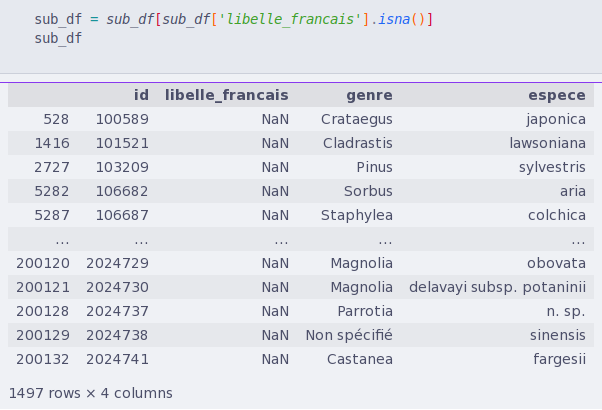
\includegraphics[width=0.8\textwidth,keepaspectratio]{ressources/df_libfr(1).png}
			\caption{DataFrame des données manquantes pour la colonne libelle francais}
	\end{figure}
\end{frame}
\begin{frame}{Libellé Français}
	\begin{columns}
	\begin{column}{0.7\textwidth}
		\begin{itemize}
			\item 1497 données manquantes
			\item Un libellé français correspond à un couple unique (genre, espece)
			\item Pour chaque donnée manquante, nous allons essayer de trouver un libellé français correspondant à un couple (genre, espece) parmis les donnée déjà présentes
		\end{itemize}
	\end{column}
	\begin{column}{0.3\textwidth}
		\begin{figure}
			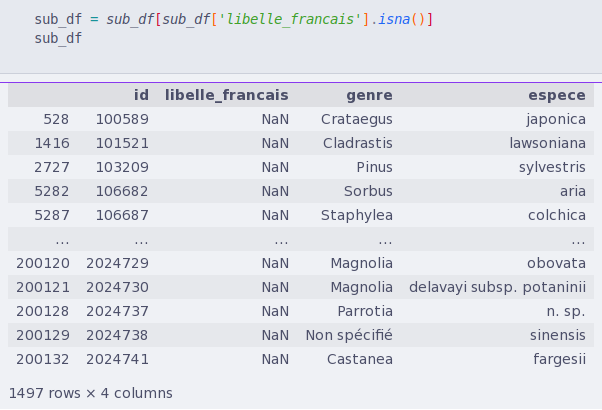
\includegraphics[width=0.8\textwidth,keepaspectratio]{ressources/df_libfr(1).png}
				\caption{DataFrame des données manquantes pour la colonne libelle francais}
		\end{figure}
	\end{column}
	\end{columns}
\end{frame}
\begin{frame}{Libellé Français}
	\begin{figure}
		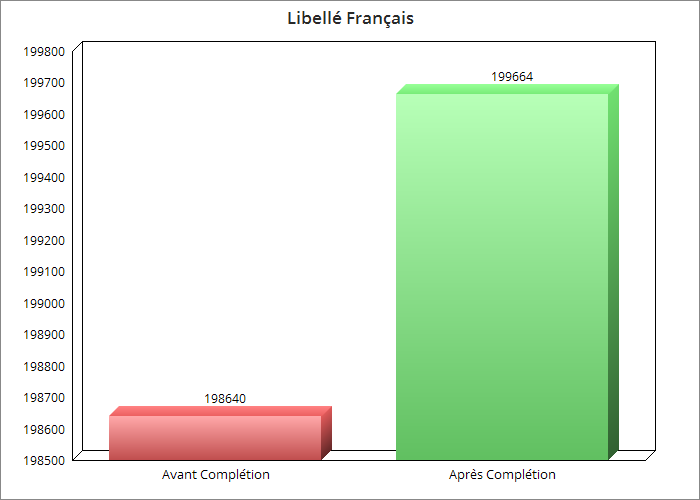
\includegraphics[width=0.6\textwidth,keepaspectratio]{ressources/libfrancais.png}
			\caption{Résultat de la recherche de libellé français correspondant à un couple (genre, espece)}
	\end{figure}
	{
	\setbeamercolor{block title}{bg=green!30,fg=black}
	\begin{block}{Résultat}
		\begin{itemize}
			\item 1024 données manquantes ont pu être retrouvées
		\end{itemize}
	\end{block}
	}
\end{frame}

\section{Détection des outliers}
\begin{frame}{Données Géographiques}
	Nous avons les coordonnées GPS de chaque arbre :
	\begin{itemize}
		\item geo point 2d a
		\item geo point 2d b
	\end{itemize}
	Nous allons utiliser l'algorithme KNN pour détecter les outliers.
\end{frame}

\begin{frame}{Données Géographiques - Paramétrage KNN}

\end{frame}

\begin{frame}{Données Géographiques -  Résultats KNN}
	\begin{figure}
		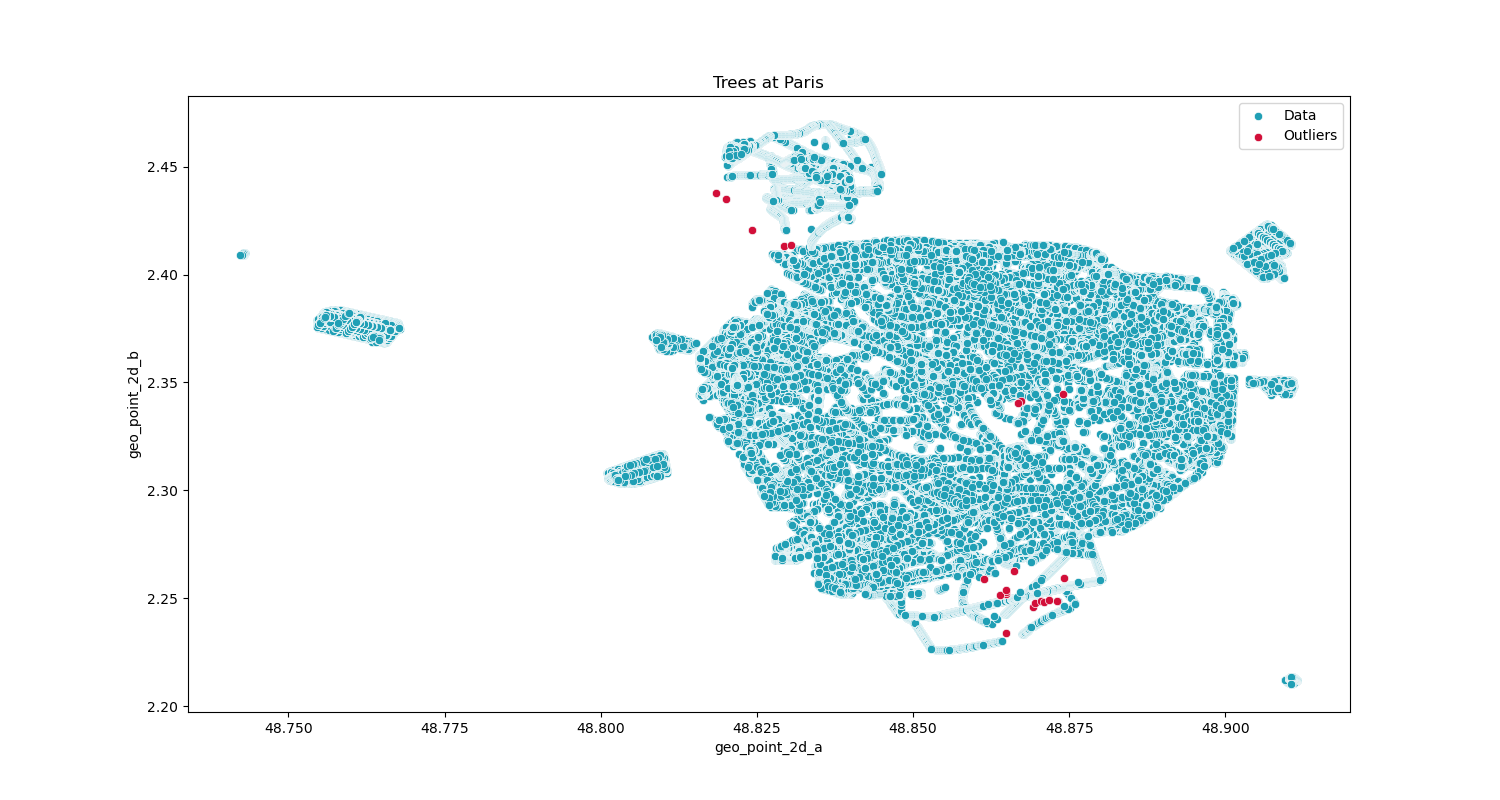
\includegraphics[width=\textwidth,keepaspectratio]{ressources/knn_outliers.png}
			\caption{Résultat de la recherche des outliers avec KNN}
	\end{figure}
\end{frame}

\begin{frame}{Données numériques de l'arbre}
	Pour chaque arbre, nous avons les données suivantes :
	\begin{itemize}
		\item hauteur
		\item circonference
	\end{itemize}
	Nous allons utiliser la méthode des interquartiles pour détecter d'éventuels outliers.
\end{frame}

\begin{frame}{Données numériques de l'arbre - IQR}
	Situation d'oringine :
	\begin{figure}
		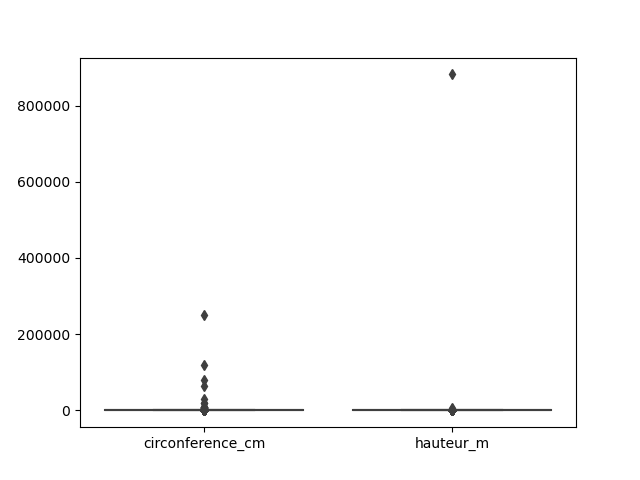
\includegraphics[width=0.65\textwidth,keepaspectratio]{ressources/boxplot_outliers.png}
		\caption{Boxplot des variables \alert{circonference} et \alert{hauteur}}
	\end{figure}
\end{frame}

\begin{frame}{Données numériques de l'arbre - IQR}
	
	\begin{itemize}
		\item $IQR = Q3 - Q1$
		\item $Limite\:basse = Q1 - 1.5 \times IQR$
		\item $Limite\:haute = Q3 + 1.5 \times IQR$
	\end{itemize}
	\begin{columns}
	\begin{column}{0.5\textwidth}
		\begin{figure}
			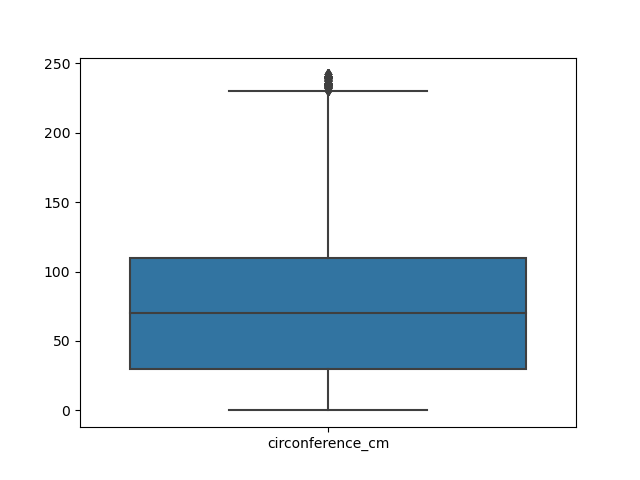
\includegraphics[width=0.8\textwidth,keepaspectratio]{ressources/boxplot_outliers_circ.png}
			\caption{Boxplot de la variable circonference après application de la méthode des IQR}
		\end{figure}
	\end{column}
	\begin{column}{0.5\textwidth}
		\begin{figure}
			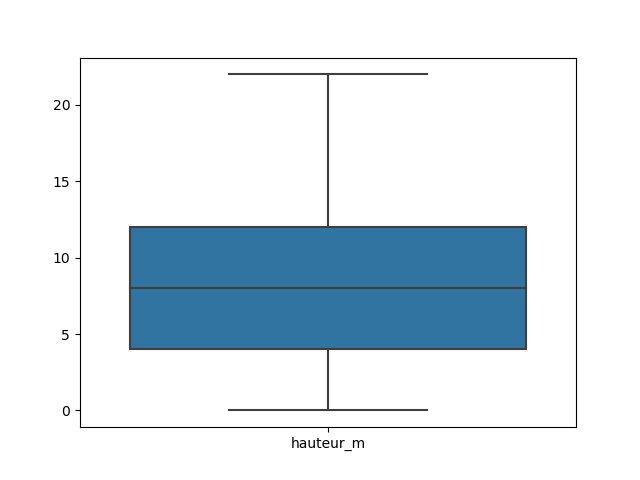
\includegraphics[width=0.8\textwidth,keepaspectratio]{ressources/boxplot_outliers_hau.png}
			\caption{Boxplot de la variable hauteur après application de la méthode des IQR}
		\end{figure}
	\end{column}
	\end{columns}
\end{frame}

\end{document}
